\documentclass[11pt,a4paper]{article}
\usepackage[margin=2.5cm]{geometry}
\usepackage{amsmath,amsfonts,amssymb}
\usepackage{graphicx}
\usepackage{hyperref}
\usepackage{booktabs}
\usepackage{enumitem}
\usepackage{tikz}
\usepackage{algorithm}
\usepackage{algpseudocode}

\title{Scenario Generator Documentation}
\author{multilayer\_milp\_gnn Benchmark}
\date{\today}

\begin{document}

\maketitle

\section{Overview}

This document explains the scenario generator implemented in 
\texttt{src/generator/generator\_v1.py} and configured by
\texttt{config/scenario\_space.yaml}. It covers:
\begin{itemize}[noitemsep]
  \item the variables that define a scenario,
  \item the allowed ranges for each parameter in the scenario space,
  \item how weather cells are constructed and how they influence the scenario, and
  \item the greedy-cover selection algorithm used to ensure diversity between scenarios.
\end{itemize}

A single scenario is represented by the \texttt{ScenarioConfig} dataclass, which aggregates:
\begin{itemize}[noitemsep]
  \item a network \emph{graph} (regions, zones, sites, interties),
  \item \emph{assets} (thermal, solar, wind, storage, hydro, demand response),
  \item an \emph{economic policy},
  \item \emph{technical scalers} for operation constraints,
  \item \emph{operation costs},
  \item \emph{exogenous} drivers (weather, demand, inflows, load-shape parameters), and
  \item a target MILP optimality gap.
\end{itemize}

\subsection{Schematic Overview}

Figure~\ref{fig:hierarchy} sketches the spatial hierarchy encoded in \texttt{GraphSpec}, while Figure~\ref{fig:exogenous} illustrates how regional weather cells and exogenous drivers combine, and Figure~\ref{fig:pipeline} summarizes the overall scenario generation pipeline.

\begin{figure}[h]
  \centering
  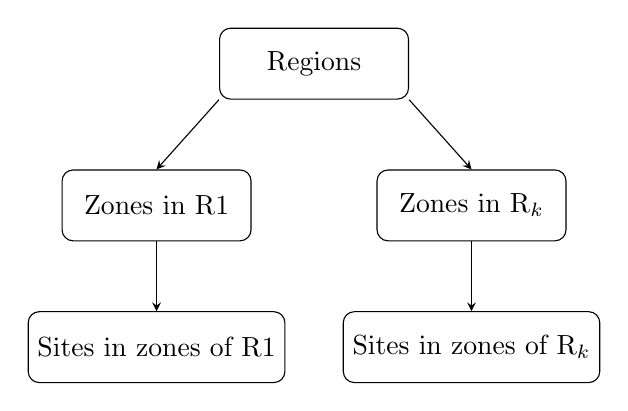
\begin{tikzpicture}[>=stealth, node distance=1.8cm]
    \tikzstyle{box}=[rectangle,draw,rounded corners,align=center,minimum width=2.4cm,minimum height=0.9cm]
    \node[box] (regions) {Regions};
    \node[box,below of=regions,xshift=-2.0cm] (zonesR1) {Zones in R1};
    \node[box,below of=regions,xshift=2.0cm] (zonesRk) {Zones in R$_k$};
    \node[box,below of=zonesR1] (sitesR1) {Sites in zones of R1};
    \node[box,below of=zonesRk] (sitesRk) {Sites in zones of R$_k$};
    \draw[->] (regions.south west) -- (zonesR1.north);
    \draw[->] (regions.south east) -- (zonesRk.north);
    \draw[->] (zonesR1.south) -- (sitesR1.north);
    \draw[->] (zonesRk.south) -- (sitesRk.north);
  \end{tikzpicture}
  \caption{Schematic spatial hierarchy: regions $\rightarrow$ zones $\rightarrow$ sites. Asset counts are sampled at site, zone or region level.}
  \label{fig:hierarchy}
\end{figure}

\begin{figure}
  \centering
  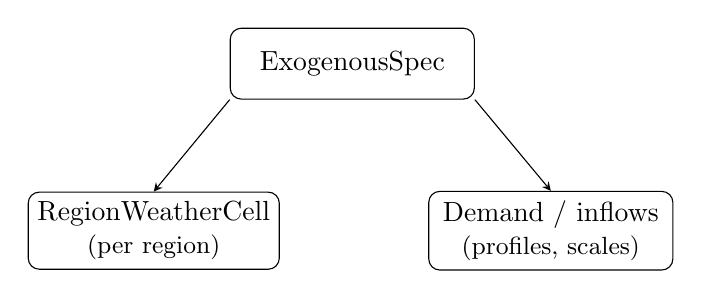
\begin{tikzpicture}[>=stealth, node distance=3cm]
    \tikzstyle{box}=[rectangle,draw,rounded corners,align=center,minimum width=3.1cm,minimum height=0.9cm]
    \node[box] (exo) {ExogenousSpec};
    \node[box,below left of=exo,xshift=-0.4cm] (weather) {RegionWeatherCell\\\small (per region)};
    \node[box,below right of=exo,xshift=0.4cm] (demand) {Demand / inflows\\\small (profiles, scales)};
    \draw[->] (exo.south west) -- (weather.north);
    \draw[->] (exo.south east) -- (demand.north);
  \end{tikzpicture}
  \caption{Exogenous layer: dominant weather profile and spread summarise per-region weather cells; demand and inflow parameters share the same exogenous block.}
  \label{fig:exogenous}
\end{figure}

\begin{figure}
  \centering
  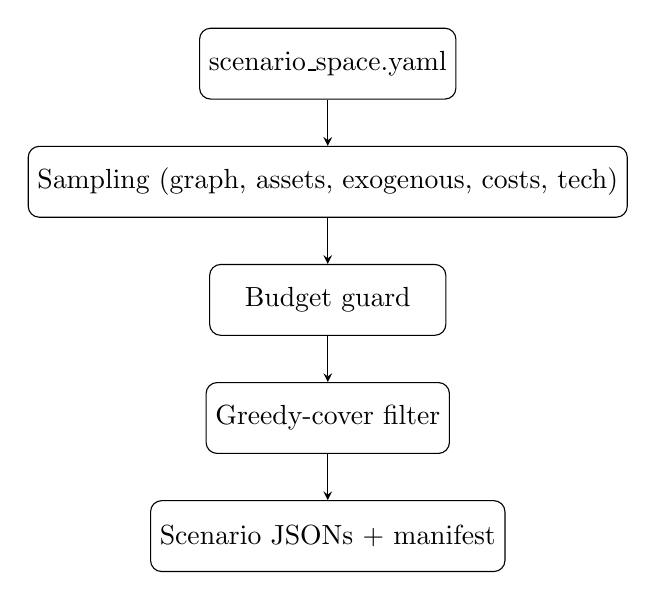
\begin{tikzpicture}[>=stealth, node distance=1.5cm]
    \tikzstyle{box}=[rectangle,draw,rounded corners,align=center,minimum width=3.0cm,minimum height=0.9cm]
    \node[box] (space) {scenario\_space.yaml};
    \node[box,below of=space] (sampling) {Sampling (graph, assets, exogenous, costs, tech)};
    \node[box,below of=sampling] (budget) {Budget guard};
    \node[box,below of=budget] (diversity) {Greedy-cover filter};
    \node[box,below of=diversity] (outputs) {Scenario JSONs + manifest};
    \draw[->] (space) -- (sampling);
    \draw[->] (sampling) -- (budget);
    \draw[->] (budget) -- (diversity);
    \draw[->] (diversity) -- (outputs);
  \end{tikzpicture}
  \caption{Scenario generation pipeline: from configuration ranges to a diverse set of accepted scenarios.}
  \label{fig:pipeline}
\end{figure}

\section{Scenario Variables and Ranges}

All numerical ranges in \texttt{scenario\_space.yaml} are inclusive bounds used to sample either integers or continuous values.

\subsection{Global Parameters}

The \texttt{global} section controls global simulation settings and the number of scenarios:
\begin{itemize}[noitemsep]
  \item \textbf{seed}: random seed (here \texttt{42}).
  \item \textbf{horizon\_hours}: total simulated horizon in hours (here \texttt{24}).
  \item \textbf{dt\_minutes}: time step in minutes (here \texttt{15}).
  \item \textbf{target\_scenarios}: desired number of accepted scenarios (here \texttt{500}).
  \item \textbf{max\_scenarios\_per\_hour\_per\_core}, \textbf{cpu\_cores}, \textbf{max\_compute\_hours}: calibration and throughput settings for the generator and solver budget.
\end{itemize}

\subsection{Network Structure}

The \texttt{structure} section describes the combinatorial structure of the network. Sampling is done by \texttt{sample\_graph}.

\begin{itemize}[noitemsep]
  \item \textbf{regions} [2, 5]: number of regions in the system.
  \item \textbf{zones\_per\_region} [3, 9]: number of zones per region. For each region, a value is drawn independently from this range.
  \item \textbf{sites\_per\_zone} [2, 8]: number of generation sites per zone. For each zone, a value is drawn from this range.
  \item \textbf{intertie\_density} [0.2, 0.6]: continuous parameter controlling the density of inter-regional ties.
  \item \textbf{neighbor\_nations} [1, 3]: number of neighboring nations, used for cross-border exchanges.
\end{itemize}

\subsection{Asset Configuration}

The \texttt{assets} section governs the asset mix, sampled by \texttt{sample\_assets}.

All of these are integer counts sampled per site, zone, or region:

\begin{itemize}[noitemsep]
  \item \textbf{thermal\_per\_site} [0, 3]
  \item \textbf{solar\_per\_site} [1, 3]
  \item \textbf{wind\_per\_site} [1, 3]
  \item \textbf{battery\_per\_site} [0, 2]
  \item \textbf{dr\_per\_site} [0, 2] (demand response).
  \item \textbf{nuclear\_per\_region} [0, 2]
  \item \textbf{hydro\_reservoir\_per\_region} [0, 3]
  \item \textbf{hydro\_ror\_per\_zone} [0, 2] (run-of-river hydro).
  \item \textbf{hydro\_pumped\_per\_region} [0, 2]
\end{itemize}

\subsection{Economic Policy}

The \texttt{economics\_policy} section is sampled by \texttt{sample\_econ}:

\begin{itemize}[noitemsep]
  \item \textbf{co2\_price\_eur\_per\_t} [35, 250]: CO$_2$ price signal.
  \item \textbf{price\_cap\_eur\_per\_mwh} [180, 4500]: price cap in the wholesale market.
  \item \textbf{cross\_border\_policy}: one of \texttt{"allow"}, \texttt{"cap"}, \texttt{"block"}.
  \item \textbf{import\_export\_caps\_factor} [0.4, 1.6]: scaling of import/export capacity.
\end{itemize}

\subsection{Technical Scalers}

The \texttt{techno\_params\_scalers} section is sampled by \texttt{sample\_tech} and governs dimensionless scalers applied to technology constraints.

\begin{itemize}[noitemsep]
  \item \textbf{thermal\_marg\_cost} [0, 15]
  \item \textbf{thermal\_ramp\_pct} [0.05, 0.45]
  \item \textbf{battery\_roundtrip\_eff} [0.78, 0.94]
  \item \textbf{battery\_e\_to\_p\_hours} [1.0, 6.0]
  \item \textbf{dr\_max\_shed\_share} [0.05, 0.35]
  \item \textbf{dr\_duration\_hours} [1, 6]
  \item \textbf{hydro\_reservoir\_head\_eff} [0.75, 1.05]
  \item \textbf{battery\_initial\_soc\_fraction} [0.35, 0.65]
  \item \textbf{battery\_final\_soc\_tolerance} [0.05, 0.18]
  \item \textbf{battery\_self\_discharge\_per\_hour} [0.001, 0.01]
  \item \textbf{pumped\_initial\_level\_fraction} [0.4, 0.7]
  \item \textbf{pumped\_final\_level\_tolerance} [0.05, 0.18]
  \item \textbf{pumped\_self\_discharge\_per\_hour} [0.0005, 0.004]
\end{itemize}

\subsection{Operation Costs}

Sampled by \texttt{sample\_operation\_costs}:

\begin{itemize}[noitemsep]
  \item \textbf{thermal\_fuel\_eur\_per\_mwh} [45, 85]
  \item \textbf{nuclear\_fuel\_eur\_per\_mwh} [8, 16]
  \item \textbf{demand\_response\_cost\_eur\_per\_mwh} [350, 1200]
  \item \textbf{value\_of\_lost\_load\_eur\_per\_mwh} [6000, 12000]
  \item \textbf{renewable\_spill\_cost\_eur\_per\_mwh} [500, 2000]
  \item \textbf{hydro\_spill\_cost\_eur\_per\_mwh} [250, 1200]
  \item \textbf{overgen\_spill\_cost\_eur\_per\_mwh} [2000, 8000]
  \item \textbf{battery\_cycle\_cost\_eur\_per\_mwh} [60, 120]
  \item \textbf{pumped\_cycle\_cost\_eur\_per\_mwh} [45, 80]
\end{itemize}

\subsection{Exogenous Drivers and Weather}

The \texttt{exogenous} section is sampled by \texttt{sample\_exogenous} and shapes weather, demand and inflows.

\begin{itemize}[noitemsep]
  \item \textbf{weather\_profiles}: a categorical list of profiles
    \texttt{"calm\_winter"}, \texttt{"stormy\_winter"}, \texttt{"sunny\_summer"}, 
    \texttt{"overcast\_summer"}, \texttt{"mixed"}.
  \item \textbf{weather\_spread\_intensity} [0.5, 1.5]: controls spatial variation within a region.
  \item \textbf{demand\_profiles}: categorical list of load profiles
    (e.g., \texttt{"wkday\_peak"}, \texttt{"wkend\_flat"}, \texttt{"cold\_snap"}, \texttt{"heatwave"}, \texttt{"shoulder"}).
  \item \textbf{demand\_scale\_factor} [0.65, 1.35]: multiplicative scaling of demand.
  \item \textbf{inflow\_factor} [0.4, 1.7]: scaling of hydro inflows.
  \item \textbf{zone\_profile\_variants}: dictionary of daily shape variants with weights.
  \item \textbf{zone\_profile\_mix\_weight} [0.4, 0.8]: range of mixture weights between variants.
  \item \textbf{zone\_profile\_phase\_shift\_hours} [-2.5, 2.5]: phase shifts of daily patterns.
  \item \textbf{zone\_profile\_noise\_std} [0.02, 0.06]: noise level applied to profiles.
  \item \textbf{zone\_profile\_curvature\_exp} [0.9, 1.18]: curvature exponent controlling peakiness.
\end{itemize}

If \texttt{zone\_profile\_variants} is omitted or invalid, default weights are used and normalized.

\subsection{Diversity and Budget Guard}

The \texttt{diversity} section configures selection of scenarios:
\begin{itemize}[noitemsep]
  \item \textbf{selection\_method}: here \texttt{"greedy\_cover"}.
  \item \textbf{cover\_metric}: list of high-level quantities used to define the meta-vector.
  \item \textbf{min\_pairwise\_distance}: minimum normalized distance between accepted scenarios (here 0.35).
\end{itemize}

The \texttt{budget\_guard} section protects against overly complex MILPs:
\begin{itemize}[noitemsep]
  \item \textbf{max\_vars\_per\_scenario}: maximum allowed variable count.
  \item \textbf{max\_cons\_per\_scenario}: maximum allowed constraint count.
  \item \textbf{mip\_gap\_target} [0.4, 1.5]: range for the target MIP gap.
  \item \textbf{time\_estimator}: coefficients used by a linear model to estimate solve time.
  \item \textbf{reject\_if\_est\_cpu\_hours\_gt}: scenarios exceeding this estimated time are rejected.
\end{itemize}

\section{Weather Cells and Scenario Creation}

Weather is represented via the \texttt{RegionWeatherCell} and \texttt{ExogenousSpec} dataclasses.

\subsection{Region Weather Cells}

For each region, the generator constructs a \emph{region weather cell}:
\begin{itemize}[noitemsep]
  \item \textbf{weather\_profile}: sampled from \texttt{weather\_profiles}.
  \item \textbf{weather\_spread\_intensity}: sampled from \texttt{weather\_spread\_intensity}.
\end{itemize}

Looping over all regions, the generator:
\begin{enumerate}[noitemsep]
  \item Draws a \emph{profile} for region $R_i$ from \texttt{weather\_profiles}.
  \item Draws a \emph{spread} value from the configured bounds.
  \item Stores these in a \texttt{RegionWeatherCell} and collects all profiles and spreads.
\end{enumerate}

After all regions are processed, it computes:
\begin{itemize}[noitemsep]
  \item the \emph{dominant} weather profile (most frequent across regions),
  \item the average spread, clipped back to the configured range.
\end{itemize}

These aggregate values are stored in the top-level \texttt{ExogenousSpec} as \texttt{weather\_profile} and \texttt{weather\_spread\_intensity}, while the per-region cells are stored in \texttt{region\_weather}.

Intuitively, the region-level cells capture spatial heterogeneity, while the dominant profile and average spread are a compact summary used downstream (for example when constructing the diversity meta-vector).

\subsection{Interaction with Demand and Inflows}

The same \texttt{ExogenousSpec} instance also contains:
\begin{itemize}[noitemsep]
  \item a \textbf{demand\_profile} chosen from \texttt{demand\_profiles},
  \item a \textbf{demand\_scale\_factor} sampled from its range,
  \item an \textbf{inflow\_factor} for hydro inflows, and
  \item parameters describing the distribution of zone-level load shapes (variants, mix range, phase, noise, curvature).
\end{itemize}

Together with region weather cells, these parameters define a coherent weather--demand--inflow scenario for the whole network. The interaction is implemented in \texttt{src/milp/scenario\_loader.py} as follows.

First, a \emph{global} base demand profile is built via
\begin{equation*}
  d^{\text{base}}(t) = \texttt{build\_demand\_profile}\bigl(\texttt{exo["demand\_profile"]}, T, \Delta t, \text{rng}\bigr),
\end{equation*}
where $T$ is the number of time steps and $\Delta t$ the time step in hours. This base profile captures the intra-day shape implied by labels such as \texttt{"wkday\_peak"}, \texttt{"cold\_snap"}, etc.

Then, a \emph{zone-specific} profile $d_z(t)$ is obtained by mixing the global profile with a randomly chosen variant, applying phase shifts, curvature and noise (function \texttt{\_make\_zone\_demand\_profile}):
\begin{equation*}
  d_z(t) = \operatorname{norm}\Bigl(\, m_z \, d^{\text{var}}_z(t + \phi_z) + \bigl(1 - m_z\bigr) d^{\text{base}}(t) + \varepsilon_z(t) \,\Bigr)^{\gamma_z},
\end{equation*}
where $m_z$ is drawn from the mix range, $d^{\text{var}}_z$ is built from one of the variants in \texttt{zone\_profile\_variants}, $\phi_z$ from the phase-shift range, $\varepsilon_z$ from the noise range, $\gamma_z$ from the curvature range, and \texttt{norm} denotes a clipping-and-normalization operator. This construction does not depend directly on the region weather cells, but it shares the same exogenous block, so changes in \texttt{ExogenousSpec} jointly affect demand, inflows and renewables.

The \textbf{demand\_scale\_factor} from \texttt{ExogenousSpec} is applied later as a multiplicative factor to the peak demand in each zone, i.e.
\begin{equation*}
  D_z(t) = \operatorname{Peak}_z\bigl(\text{exo}\bigr) \cdot d_z(t),
\end{equation*}
where \(\operatorname{Peak}_z\) itself depends on \texttt{demand\_scale\_factor} and a small amount of zone-specific randomness.

For hydro, two distinct exogenous channels are used:
\begin{itemize}[noitemsep]
  \item a \emph{run-of-river} profile \(r(t)\) built as \texttt{build\_runofriver\_profile(T, \,$\Delta t$,\, avg\_region\_spread,\, rng)}, where \texttt{avg\_region\_spread} is the average of the per-region spreads from the weather cells;
  \item an \emph{inflow} profile \(i(t)\) for reservoir hydro built as \texttt{build\_inflow\_profile(T, \,$\Delta t$,\, inflow\_factor,\, rng)}, directly driven by \texttt{ExogenousSpec.inflow\_factor}.
\end{itemize}
The run-of-river profile thus inherits variability from regional weather spreads, while the longer-term inflow trend is modulated by \texttt{inflow\_factor}.

Overall, the exogenous block couples demand, run-of-river and inflows to the same scenario-level random seed and configuration, while the weather cells provide spatially resolved intensity signals used mainly for renewables, as detailed next.

\subsection{Weather-Driven Renewable Generation Profiles}

The region weather cells play a central role in constructing solar and wind availability profiles. In \texttt{load\_scenario\_data}, the map \texttt{exogenous.region\_weather} is first decoded into two per-region arrays:
\begin{itemize}[noitemsep]
  \item \texttt{region\_weather\_profile[R]}: the weather profile name for region $R$ (e.g. \texttt{"sunny\_summer"}, \texttt{"stormy\_winter"});
  \item \texttt{region\_weather\_spread[R]}: the non-negative spread intensity for region $R$.
\end{itemize}

For each region $R$, two \emph{base} renewable time series are generated using the weather-driven profile name and spread:
\begin{align*}
  s_R(t) &= \texttt{build\_solar\_profile}\bigl(\texttt{region\_weather\_profile[R]}, T, \Delta t, \text{rng}_R^{(\text{solar})}, \texttt{region\_weather\_spread[R]}\bigr), \\
  w_R(t) &= \texttt{build\_wind\_profile}\bigl(\texttt{region\_weather\_profile[R]}, T, \Delta t, \text{rng}_R^{(\text{wind})}, \texttt{region\_weather\_spread[R]}\bigr).
\end{align*}
The functions \texttt{build\_solar\_profile} and \texttt{build\_wind\_profile} implement stylized diurnal and mesoscale patterns whose amplitude, cloudiness and gustiness are modulated by the \emph{intensity} argument (fed here by \texttt{weather\_spread\_intensity}). High-spread regimes lead to more volatile profiles with stronger noise and shading/lull episodes.

At the zone level, these regional bases are perturbed to obtain zone-specific renewable availability profiles:
\begin{itemize}[noitemsep]
  \item each zone is mapped to a region $R$, inheriting \texttt{region\_weather\_profile[R]} and \texttt{region\_weather\_spread[R]};
  \item a scaling factor and additive Gaussian noise with variance proportional to the spread are applied to the regional solar profile $s_R(t)$;
  \item for wind, additional random temporal shifts (a few time steps forward or backward) and noise are applied to $w_R(t)$, again with scale tied to the spread.
\end{itemize}

Formally, for a zone $z$ in region $R$ one obtains
\begin{align*}
  S_z(t) &= \operatorname{clip}\bigl( \alpha_z \, s_R(t) + \eta^{(\text{solar})}_z(t; \sigma_R),\, 0, 1 \bigr), \\
  W_z(t) &= \operatorname{clip}\bigl( \operatorname{shift}_{k_z} w_R(t) + \eta^{(\text{wind})}_z(t; \sigma_R),\, 0, 1 \bigr),
\end{align*}
where $\alpha_z$ is a zone-specific scale (around unity), $\sigma_R$ depends on \texttt{region\_weather\_spread[R]}, $k_z$ is an integer time shift, and $\eta$ denotes Gaussian noise. These dimensionless profiles are subsequently multiplied by the installed solar and wind capacities in each zone to yield available renewable power.

In summary, the weather cells define a coarse-grained regional climate state (profile name) and an associated variability level (spread). This pair is:
\begin{itemize}[noitemsep]
  \item used directly to synthesize region-level solar and wind base profiles;
  \item propagated to zones via stochastic scaling, shifting and noise;
  \item indirectly reflected in run-of-river and, through the exogenous block, coordinated with demand and reservoir inflows.
\end{itemize}

\section{Greedy-Cover Diversity Selection}

\subsection{Scenario Generation Loop}

The main generator function \texttt{generate\_scenarios} repeats the following steps until it either reaches the target number of scenarios or hits a maximum number of attempts:

\begin{enumerate}[noitemsep]
  \item Sample \textbf{graph}, \textbf{assets}, \textbf{economic policy}, \textbf{technical scalers}, \textbf{costs} and \textbf{exogenous} variables from the space.
  \item Sample a \textbf{MIP gap target} from \texttt{mip\_gap\_target}.
  \item Build a \texttt{ScenarioConfig} instance.
  \item Estimate MILP size and solve time, reject if the budget guard is violated.
  \item Apply the greedy-cover diversity filter (if enabled).
  \item If accepted, write the scenario JSON file and record its metadata.
\end{enumerate}

\subsection{Meta-Vector Construction}

For each candidate scenario, a \emph{meta-vector} $v$ is built by \texttt{scenario\_meta\_vector}. This vector contains:

\begin{itemize}[noitemsep]
  \item structural features: number of regions, average zones per region, intertie density;
  \item economic features: CO$_2$ price, price cap;
  \item exogenous scalars: demand scale factor;
  \item asset intensity: average solar and wind units per site;
  \item load-shape mix range: lower and upper bounds of \texttt{zone\_profile\_mix\_weight};
  \item key operation costs: thermal, nuclear, demand response, value of lost load, renewable/hydro/overgeneration spill costs;
  \item one-hot encoding of the dominant weather profile; and
  \item one-hot encoding of the cross-border policy.
\end{itemize}

Formally, categoricals (weather profile and cross-border policy) are turned into one-hot sub-vectors and concatenated to the numerical part.

For a given scenario $s$, we denote its meta-vector by $v(s) \in \mathbb{R}^d$ after concatenation of all components listed above.

\subsection{Distance and Normalization}

To compare scenarios, the generator uses a normalized Euclidean distance:
\begin{equation}
  d(a,b) = \left\Vert \frac{a - b}{\max(\text{maxs} - \text{mins}, 10^{-9})} \right\Vert_2,
\end{equation}
where \texttt{mins} and \texttt{maxs} are per-dimension lower and upper bounds derived from the scenario space, and the division is element-wise.

This means each dimension is rescaled to $[0,1]$ (approximately) before computing the Euclidean norm, so that parameters with larger numeric ranges do not dominate the distance.

\subsection{Greedy-Cover Rule}

Let $V$ be the set of meta-vectors for already accepted scenarios, and let $v$ be the meta-vector for the current candidate. The greedy-cover rule is:

\begin{itemize}[noitemsep]
  \item If $V$ is empty, accept the candidate and add $v$ to $V$.
  \item Otherwise, compute distances $d(v, v')$ for all $v' \in V$ and let $d_{\max}$ be their maximum.
  \item If $d_{\max} < d_{\min}$ (where $d_{\min}$ is \texttt{min\_pairwise\_distance}), reject the scenario.
  \item Otherwise, accept it and add $v$ to $V$.
\end{itemize}

With \texttt{min\_pairwise\_distance = 0.35}, each new scenario must be sufficiently far, in this normalized feature space, from \emph{all} previously accepted scenarios. This is a greedy algorithm because it:

\begin{itemize}[noitemsep]
  \item considers scenarios one by one in the order they are sampled, and
  \item never revisits or swaps earlier decisions.
\end{itemize}

The result is a diverse set of scenarios spread across the configuration space, subject to the constraints imposed by the budget guard.

\subsection{Formalization and Pseudocode}

Let $S$ be the (potentially infinite) set of candidate scenarios produced by the sampling process, and let $A \subset S$ be the set of accepted scenarios. Given a distance threshold $d_{\min} > 0$, the greedy-cover algorithm can be written as the iterative update
\begin{equation}
  A_{k+1} =
  \begin{cases}
    A_k \cup \{s_k\} & \text{if } \max_{s \in A_k} d\bigl(v(s_k), v(s)\bigr) \ge d_{\min}, \\\\
    A_k & \text{otherwise},
  \end{cases}
\end{equation}
where $s_k$ is the $k$-th candidate that passes the budget guard and $d(\cdot,\cdot)$ is the normalized distance.

Equivalently, the acceptance condition can be expressed as a constraint on the feasible region in feature space:
\begin{equation}
  v(s_k) \in \mathcal{V} \setminus \bigcup_{s \in A_k} B\bigl(v(s), d_{\min}\bigr),
\end{equation}
where $\mathcal{V} \subseteq \mathbb{R}^d$ is the domain of meta-vectors and $B(v, r)$ denotes the closed Euclidean ball of radius $r$ centred at $v$.

Algorithm~\ref{alg:greedy-cover} summarizes the implementation in \texttt{generate\_scenarios}.

\begin{algorithm}[h]
  \caption{Greedy-cover scenario selection with budget guard}
  \label{alg:greedy-cover}
  \begin{algorithmic}[1]
    \Require configuration space \texttt{space}, target size $T$, minimum distance $d_{\min}$
    \State $A \gets \emptyset$ \Comment{accepted scenarios}
    \State $V \gets [\ ]$ \Comment{list of meta-vectors}
    \State $n \gets 0$; $\text{attempts} \gets 0$
    \While{$n < T$ and $\text{attempts} < 25 T$}
      \State $\text{attempts} \gets \text{attempts} + 1$
      \State sample $\text{graph}, \text{assets}, \text{econ}, \text{tech}, \text{costs}, \text{exo}$ from \texttt{space}
      \State construct scenario $s$ and compute MILP size estimates $\text{vars}, \text{cons}$
      \State estimate solve time $t$ and \textbf{continue} if budget guard rejects $(\text{vars}, \text{cons}, t)$
      \If{$\texttt{selection\_method} = "greedy\_cover"$}
        \State compute meta-vector $v \gets v(s)$
        \If{$V \neq \emptyset$}
          \State compute $d_{\max} \gets \max_{w \in V} d(v, w)$
          \If{$d_{\max} < d_{\min}$}
            \State \textbf{continue} \Comment{reject; too similar to existing scenarios}
          \EndIf
        \EndIf
        \State append $v$ to $V$
      \EndIf
      \State accept $s$: add to $A$ and write scenario JSON
      \State $n \gets n + 1$
    \EndWhile
    \State \Return $A$ and manifest statistics
  \end{algorithmic}
\end{algorithm}

\section{Outputs}

For each accepted scenario, the generator writes:
\begin{itemize}[noitemsep]
  \item a JSON file \texttt{scenario\_XXXXX.json} containing the full \texttt{ScenarioConfig} plus metadata and estimates;
  \item a \texttt{manifest.json} summarizing total counts, attempts, and aggregate statistics.
\end{itemize}

The manifest records, among others, average regions, zones, sites, variable and constraint counts, and estimated CPU hours under the time estimator.

\section{Example Generated Scenario}

To make the abstract description above more concrete, this section summarizes one representative generated scenario (file \texttt{scenario\_00001.json} in \texttt{outputs/scenarios\_v1}). We do not reproduce the raw JSON, but instead highlight the key values and relate them to the configuration ranges.

\subsection{Graph and Assets}

In this example, the graph has:
\begin{itemize}[noitemsep]
  \item $2$ regions,
  \item zones per region given by $[3, 8]$, for a total of $11$ zones,
  \item $11$ sites (one or more per zone),
  \item intertie density $0.369$ (within the configured range $[0.2, 0.6]$),
  \item $1$ neighbouring nation.
\end{itemize}

Asset counts are consistent with the ranges defined in the asset block: e.g., thermal units per site lie in $[0,3]$, solar in $[1,3]$, wind in $[1,3]$, batteries in $[0,2]$, and so on. Aggregated counts for this scenario (as stored in the meta-section) are:
\begin{itemize}[noitemsep]
  \item $13$ thermal units, $18$ solar units, $22$ wind units,
  \item $14$ battery units, $7$ demand-response resources,
  \item $2$ nuclear plants, $3$ reservoir hydro units,
  \item $14$ run-of-river hydro units, $2$ pumped-hydro units.
\end{itemize}

\subsection{Economic Policy and Technical Parameters}

The economic policy for this scenario is:
\begin{itemize}[noitemsep]
  \item CO$_2$ price: approximately \texttt{93 EUR/t} (within $[35,250]$),
  \item price cap: about \texttt{4178 EUR/MWh} (within $[180,4500]$),
  \item cross-border policy: \texttt{"block"},
  \item import/export caps factor: about \texttt{1.07}.
\end{itemize}

Technical scalers and operation costs are similarly sampled within their respective ranges. For instance, the thermal marginal cost scaler is about \texttt{10.27}, the battery round-trip efficiency is around \texttt{0.90}, and the value of lost load is approximately \texttt{7480 EUR/MWh}.

\subsection{Exogenous Drivers and Weather}

The exogenous block for this scenario reads:
\begin{itemize}[noitemsep]
  \item dominant weather profile: \texttt{"stormy\_winter"},
  \item weather spread intensity: about \texttt{1.25},
  \item demand profile: \texttt{"wkday\_peak"},
  \item demand scale factor: about \texttt{1.18},
  \item inflow factor: about \texttt{1.52}.
\end{itemize}

Zone-level profile variants and their weights match the defaults from \texttt{scenario\_space.yaml}. The mix-weight range is exactly $[0.4,0.8]$, with phase shifts, noise and curvature parameters at their configured ranges.

Per-region weather cells are:
\begin{itemize}[noitemsep]
  \item Region R1: profile \texttt{"stormy\_winter"} with spread $\approx 1.50$,
  \item Region R2: profile \texttt{"stormy\_winter"} with spread $\approx 1.01$.
\end{itemize}
The dominant profile is thus \texttt{"stormy\_winter"}, and the average spread (clipped to $[0.5,1.5]$) yields the reported exogenous spread intensity.

\subsection{Complexity Estimates and Meta-Vector}

For this scenario, the estimated MILP size is about \texttt{53k} variables and \texttt{69k} constraints, with an estimated solve time slightly above one CPU-hour under the configured time estimator. These values fall below the budget-guard thresholds, so the scenario is eligible for the diversity filter.

The meta-section of the JSON file stores the meta-vector components used by the greedy-cover algorithm: structural counts (regions, zones, sites), aggregated asset counts, demand scale factor, operation costs, technical scalers, weather profile and cross-border policy. When normalized by \texttt{mins} and \texttt{maxs}, this vector is required to be at least a distance $d_{\min}=0.35$ away from all previously accepted scenarios in order to be included in the final set.

This example illustrates how the abstract configuration ranges materialize as a concrete, self-consistent scenario instance.

\end{document}
